\documentclass{article}
\usepackage[utf8]{inputenc}
\usepackage{hyperref}
\usepackage{graphicx}
\usepackage{float}
\usepackage{listings}

\title{Assignement 3}
\author{Iván Piña Arévalo \\ ivan.pinaarevalo@alum.uca.es}
\date{\today}

\begin{document}
\maketitle

\newpage
\begin{abstract}
    En esta práctica, realizaremos la implementación de una reducción polinomica. 
    Concretamente, reduciremos el problema del coloreado de un grafo al problema
    3-SAT. Una vez implementado nuestro programa, realizaremos análisis sobre su 
    complejidad termporal, así como las relaciones entre el número de colores 
    necesarios y el máximo clique del grafo. Se ha empleado el grafo de Petersen.
\end{abstract}

\newpage

\section{Introduction}
    En primer, lugar, comenzaremos hablando del coloreado de un grafo. Este problema
    consiste en colorear un grafo de tal manera que dos vértices adyacentes no pueden 
    tener el mismo color. 
    %¿Qué tipo de problema es este? Es de la clase NP-complete
    %Insertar el primer grafo de ejemplo.
    \begin{figure}[H]
        \centering
        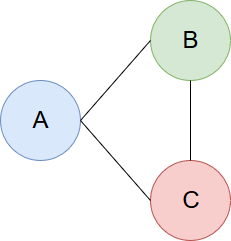
\includegraphics[width=0.5\textwidth]{pictures/ejemplo.png}
        \caption{twitterProductor.py}
    \end{figure}
	
    \begin{figure}[H]
        \centering
        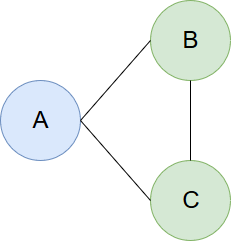
\includegraphics[width=0.5\textwidth]{pictures/ejemplobad.png}
        \caption{twitterProductor.py}
    \end{figure}

	Concretamente, hemos empleado el grafo de Petersen

    \begin{figure}[H]
        \centering
        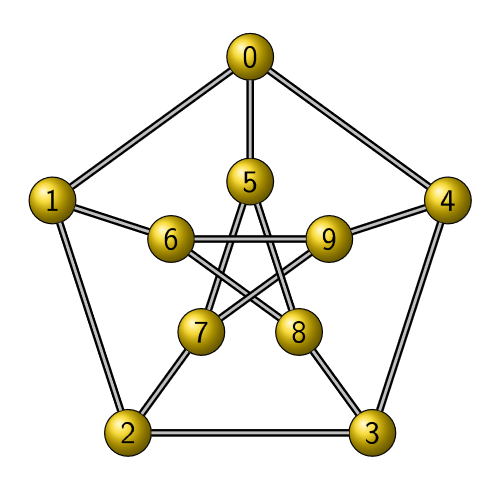
\includegraphics[width=0.5\textwidth]{pictures/PetersenGraph.png}
        \caption{twitterProductor.py}
    \end{figure}

    Para encontrar la solución de este problema se ha empleado el problema 3-SAT. 
    %Explicar que es el problema 3-SAT
    El problema SAT fue uno de los primers en descubrirse NP-completo. Dicho problema consiste 
    en dada una ecuación booleana, encontrar los valores para los cuales es verdadera. Además, la 
    ecuación debe tener las siguientes características: 
    \begin{itemize}
        \item La ecuación global se compone de ecuaciones enlazadas con la puerta logica and
        \item Cada subecuación esta compuesta por variables ($x_1, x_2, ...$) unidas por la puerta lógica OR.
    \end{itemize}

    A continuación podemos ver una ecuación para el problema SAT:
        \[ ( x_1 \vee x_2 \vee x_3) \wedge (x_3 \vee x_4)\]

    
\section{Methodology}
    La implementación de la práctica se ha realizado en C++, hemos dividido el programa en varias partes.
    \subsubsection{Lectura del grafo}
        Para la lectura del grafo nos hemos apoyado en un fichero. Dicho fichero debe tener la siguiente estructura:
        \begin{itemize}
            \item La definición de cada nodo se realiza en una fila. 
            \item Los nodos a los que esta conectado el nodo que estamos definiendo estan separados por comas. 
        \end{itemize}
        
        De esta manera realizamos la lectura del grafo, representado mediante listas de adyacencia.
        A continuación podemos ver el fichero con el grafo de ejemplo de la sección anterior.
        %Insertar fichero con el grafo de ejemplo.
    
    \subsubsection{Transformación del 3-Col to SAT}
        Lo primero al realizar esta parte ha sido analizar profundamente la estructura de las ecuaciones booleanas que 
        representan al grafo que deseamos colorear.
        Estas ecuaciones se pueden dividir en dos grupos.
        \begin{itemize}
            \item Ecuaciones correspondientes al color del propio nodo.
            \item Ecuaciones correspondientes al color de los nodos adyacentes al nodo actual.
        \end{itemize}
        %Remarcar que por eficiencia temporal las aristas se escriben dobles, cosa que no afecta a picosat.
    
    \subsubsection{Escritura de las ecuaciones booleanas}
        Finalmente es necesario escribir en un fichero las ecuaciones correspondientes al grafo. Estas 
        ecuaciones deben ir en formato DIMACS. El fin de este formato es el correcto procesamiento por parte del 
        programa PicoSAT. 

        Simplemente en lugar de ir mostrando las ecuaciones por la salida estándar las hemos dirigido hacia una cadena. Igualmente 
        hemos definido una variable que se encarga de contar cuantas ecuaciones tiene y otra más para el número de variables. 
        Volcando las cadenas y los contadores en un fichero conseguimos tener la información lista para PicoSAT.

        El programa ha sido paramétrizado de tal forma que tanto el grafo como el número de colores pueda modificarse. 
    
    \subsubsection{PicoSAT}
        Finalmente, para ejecutar el programa hemos empleado la orden: 
        \[./picosat salida\]

        Si deseamos ver todas las soluciones 
        \[./picosat --all salida\]


\section{Results and Discussion}
    Para averiguar el tipo de reducción obtenida hemos realizado un estudio de la complejidad temporal del programa: 
        %Estudio teorico. 
    Por lo tanto, nuestro programa posee una complejidad polinómica. Consecuentemente hemos obtenido una reducción polinómica.
    Una solución para el grafo de Petersen es esta: 

    Así mismo, todas las posibles soluciones son: 
        %Insertar la solución de las ecuaciones booleanas, no te compliques coloreando el grafo.
    
    Analizando el grafo, concluimos que el Clique Máximo del grafo de Petersen es de tamaño 2. Por ejemplo: 
        %Mostrar un clique de tamaño 2 en el grafo de Petersen. 
    
    


\section{Conclussion}
\bibliography{bibliografia} 
\bibliographystyle{unsrt}

\end{document}
